\documentclass[8pt]{report}
\usepackage{amsmath, xfrac, enumitem, graphicx, ulem, float, bigints, bm, textcomp}
\usepackage{titlesec, mathtools}
\usepackage[margin=0.7in]{geometry}
\graphicspath{ {images/} }
\linespread{0.8}
\title{\Huge{\textsc{Mathematics - GATE}}}
\author{\huge{\textbf{Kulasekaran}}}
\begin{document}
\maketitle
\tableofcontents
\chapter{Linear Algebra}
%-----------------------------------------------------------------------------------------%
\chapter{Differential and Integral Calculus}
%-----------------------------------------------------------------------------------------%
\chapter{Vector Calculus}
%-----------------------------------------------------------------------------------------%
\chapter{Differential Equations}
%-----------------------------------------------------------------------------------------%
\chapter{Probability and Statistics}
\section{Introduction and Basics}
	\begin{itemize}
		\item \textbf{Random Experiment} : An experiment in which the result is unpredictable, but the possibilities of the result is known. Eg. When you throw a coin, you don't know its gonna be head or tail. But you know it will be either one of them.
		\item \textbf{Sample Space(S)} : A set of all possible outcomes of a random experiment is called its sample space. For the above mentioned coin toss example the sample space is s:\{H,T\} $\boxed{P(s)=1}$
		\item \textbf{Event} : A subset of the sample space is called as event. For the above mentioned example, the event can be in which the coin lands as H, or the event can be in which the coin lands as tail. Another example: Throwing a fair dice, S=\{1,2,3,4,5,6\}. An event can be in which the number on the top of the dice will be even, So $\implies$ \{2,4,6\}. $\boxed{0\le P(E)\le1}$
		\begin{itemize}
			\item \textbf{Simple event:} Only one element is possible in the event. Eg. coin toss $\implies$ \{H\} or \{T\}
			\item \textbf{Compound event:} More than one element is possible in the event. Eg. Even number on the dice top.
		\end{itemize}
		 \item \textbf{Union}$\pmb{(\cup)}$ Let S=\{1,2,3,4,5,6,7,8,9,10\} If three events are described,say: 
		 	\begin{itemize}
		 		\item A = should be a multiple of 2 = \{2,4,6,8,10\}
		 		\item B = should be a multiple of 3 = \{3,6,9\}
		 		\item C = Either a multiple of 2 or 3 = \{2,3,4,6,8,9,10\}
		 		\item The event C can be written as $\pmb{(A\cup B)}$ as it contains all the elements in A as well as all the elements in B
		 	\end{itemize}
		 \item \textbf{Intersection}$\pmb{(\cap)}$ For the same sample space mentioned above, let there be a fourth event D such that D = should be a multiple of both 2 and 3 = \{6\}. Then D can be written as $\pmb{(A\cap B)}$
		 \begin{figure}[H]
		 		\centering
		 		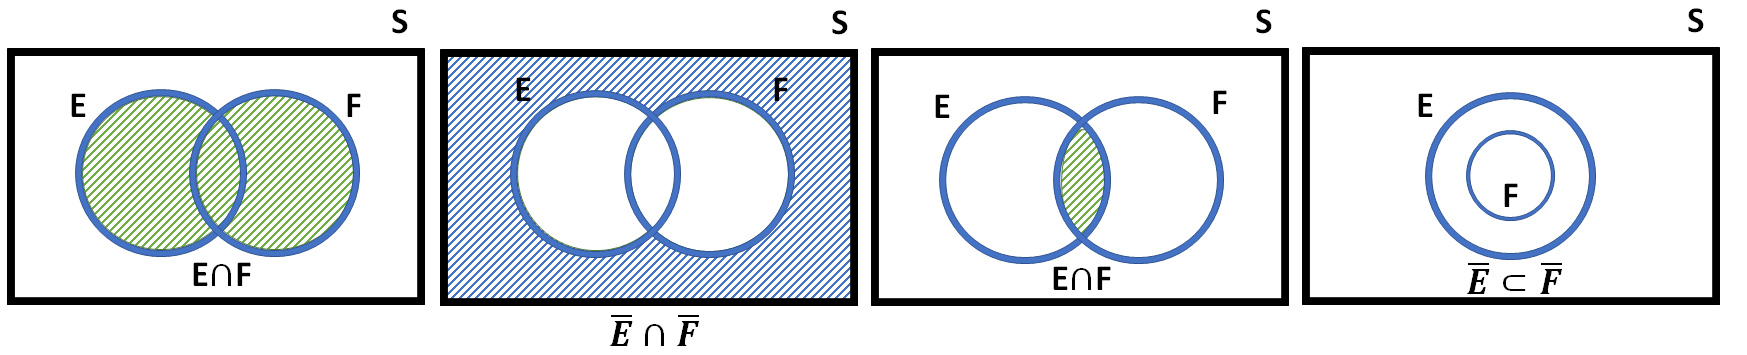
\includegraphics[scale=0.4]{Setrepresentation.png}
		 \end{figure}
		 \item \textbf{Permutations($^nP_r$)}
		 	\begin{itemize}
		 		\item Permutation means \textbf{Arrangement} $\boxed{^nP_r = \dfrac{n!}{(n-r)!}} \impliedby$ (Ways to arrange r things out of n things)
		 	\end{itemize}
		 \item \textbf{Combinations($^nC_r$)}
		 	\begin{itemize}
		 		\item Combination means \textbf{Selection} $\boxed{^nC_r = \dfrac{n!}{(n-r)!r!} = \dfrac{^nP_r}{r!}}\impliedby$ (Ways to select r things out of n things)
		 	\end{itemize}
	\end{itemize}\hrulefill
%-----------------------------------------------------------------------------------------%
	\section{Types of Events}
	\subsection{Complementary events}
		\begin{itemize}
			\item If S=\{1,2,3,4,5\} and A = even numbers - \{2,4\}, then the complimentary even of A is denoted by $\bar{A}$=\{1,3,5\}
		\end{itemize}
%-----------------------------------------------------------------------------------------%
	\subsection{Equally likely events}
		\begin{itemize}
			\item Two events are equally likely events when the probability for both the events are same. For Eg. Getting a head or a tail on a coin toss is 50/50
		\end{itemize}
%-----------------------------------------------------------------------------------------%
	\subsection{Mutually Exclusive events}
		\begin{itemize}
			\item Two events are mutually exclusive if when one event occurs, the other cannot occur simultaneously. For eg. you can get only a head or a tail but not both on a coin toss on a single try.
			\item $\boxed{p(E_1\cup E_2)=p(E_1)+p(E_2)}\impliedby$ ($E_1$ and $E_2$ are mutually exclusive) $\implies\boxed{p(E_1\cap E_2) = 0}$
		\end{itemize}
%-----------------------------------------------------------------------------------------%
	\subsection{Collectively Exhaustive events}
		\begin{itemize}
			\item If the union of two events give the sample space, then they are called collectively exhaustive events
		\end{itemize}
%-----------------------------------------------------------------------------------------%
	\subsection{Independent events}
		\begin{itemize}
			\item When the occurrence of one event doesn't affect the occurrence of another event. For eg. In a bag of 5 red balls and 3 black balls, if two balls are drawn at random one at a time \textbf{with replacement}, then the probability of getting say 2 red balls is not affected by whether you got red ball on the first pick or not. 
			\item If it had been \textbf{without replacement}, then the probability will change
			\item If two events are independent, then conditional probability becomes marginal probability 
			\item $\implies p(A/B) = p(A),\;\;p(B/A) = p(B)\;\;\;\boxed{p(A\cap B) = p(A)*p(B)}$
		\end{itemize}\hrulefill
%-----------------------------------------------------------------------------------------%
\section{De Morgan's Law}
	\begin{itemize}
		\item $\boxed{\overline{(E_1\cup E_2)} = (\bar{E_1}\cap \bar{E_2})}\;\;\;\boxed{(\overline{E_1\cap E_2)} = (\bar{E_1}\cup \bar{E_2})}\;\;\;$ $\boxed{p(\bar{E_1}\cap \bar{E_2})\;i.e.,(\;Neither\;E_1\;nor\;E_2) = 1 - p(E_1\cup E_2)}$
	\end{itemize}\hrulefill
%-----------------------------------------------------------------------------------------%
\section{Approaches to Probability}
	\subsection{Classical Approach}
		\begin{itemize}
			\item $\boxed{p(E) = \dfrac{n(E)}{n(S)}}\impliedby$ (Classical approach assumes that all outcomes are equally likely)
		\end{itemize}\hrulefill
%-----------------------------------------------------------------------------------------%
\section{Rules of Probability}
	\begin{enumerate}
		\item $\boxed{p(A\cup B)=p(A)+p(B)-p(A\cap B)}\impliedby$ \textbf{(Inclusion-Exclusion rule)}
		\item $\boxed{p(A\cup B) = p(A)*p(B/A) = p(B)*p(A/B)\impliedby}$ \textbf{(Conditional Probability)}
			\begin{itemize}
				\item Here, p(A) and p(B) are called \textsc{Marginal probabilities}
				\item p(A/B) and p(B/A) are called \textsc{Conditional probabilities}
				\item p(A/B) = Probability of occurrence of A when B has already occurred
				\item p(B/A) = Probability of occurrence of B when A has already occurred
				\item Conditions for three events A,B,C to be independent:
					\begin{itemize}
						\item \fbox{p(ABC) = p(A)p(B)p(C)} \fbox{p(AB) = p(A)p(B)} \fbox{p(BC) = p(B)p(C)} \fbox{p(AC) = p(A)(C)}
					\end{itemize}
			\end{itemize}
		\item $\boxed{p(A)=1-p(\bar{A})}\;\;\;\boxed{p(A)+p(\bar{A})=1}\impliedby$ \textbf{(Complimentary probability)}
		\item $\boxed{p(A/B)=\dfrac{p(A\cap B)}{p(B)}}\;\;\;\boxed{p(B/A)=\dfrac{p(A\cup B)}{p(A)}}\impliedby$ \textbf{(Conditional probability - multiplication rule)}
		\item $\boxed{p(E) = p(A\cap E)+p(B\cap E) = p(A)*(p(E/A)+p(B)*p(E/B))}\impliedby$ \textbf{(Total probability)}
			\begin{itemize}
				\item If an event E can occur in two ways A and B, then the total probability for the occurrence of E is the sum the probability of it happening by A and the probability of E happening by B.
			\end{itemize}
		\item $\boxed{p\left(E_i/A\right) = \dfrac{p(E_i\cap A)}{A} = \dfrac{p(E_i)*p(E_i/A)}{\sum_{k=1}^{n}p(E_k).p(A/E_k)}} \impliedby$ \textbf{(Baye's Theorem)}
	\end{enumerate}\hrulefill
%-----------------------------------------------------------------------------------------%
	\section{Statistics}
		\subsection{Basics and Introduction}
%-----------------------------------------------------------------------------------------%
\chapter{Numerical Methods}
%-----------------------------------------------------------------------------------------%
\chapter{Complex Numbers}
%-----------------------------------------------------------------------------------------%
\chapter{Transform Theory}
%-----------------------------------------------------------------------------------------%
%-----------------------------------------------------------------------------------------%
\end{document}
%-----------------------------------------------------------------------------------------%
%-----------------------------------------------------------------------------------------%
%-----------------------------------------------------------------------------------------%
